\chapter{Methods}\label{methods}
Summarizing the key points made in chapter \ref{background}, current deep learning pipelines are not equipped with evaluation methods suitable for out-of-distribution generalization, are largely incapable of reliably learning causally robust features, and are underspecified by the datasets they are trained on. Addressing generalization failure requires mitigating some of these problems. The literature, in broad strokes, tackles this by improving the models' inductive biases, e.g through attention-based mechanisms \cite{attention_generalizability, reverse_attention}, ensembles \cite{divergentnets, endoensemble}, etc, or their support, e.g through data augmentation techniques \cite{polyp_augmentation, cyclegan}. 

This thesis attempts to combine the central ideas behind these methods into one unified deep learning pipeline, intended primarily to maximize generalizability. The contributions can be summarized as follows:

\begin{itemize}
    \item A modified DeepLabV3-based model with dual decoders, intended to constrain the space of latent represent ations such that underspecification is mitigated
    \item A new view of generalization as consistency with respect to a hidden perturbation model and a corresponding training procedure, metric and loss-function
    \item An augmentation strategy informed by this alternative view, including both conventional augmentation functions and a \gls{gan}-inpainter decoder
    \item An family of ensembles consisting of predictors being trained according to the above methods
\end{itemize}



\section{DD-DeepLabV3+}
As described in Chapter \ref{background}, generalization failure can in part be attributed to the fact that most deep learning models are underspecified by the training data. In other words, the same pipeline can return any number of risk-equivalent predictors that leverage dramatically different features. To mitigate this, one may impose constraints on the space of features that a given model can learn, such as multi-task learning \cite{ddanet}, attention-mechanisms \cite{attention_generalizability, reverse_attention}, preprocessing \cite{visual_cortex}, etc. 

As testing the relative effectiveness of all of these different approaches is beyond the scope of this thesis, a simple model is instead introduced, namely a dual-decoder DeepLabV3+. As its name suggests, this model is functionally equivalent to a standard DeepLabV3+, but is endowed with an additional decoder, which performs image reconstruction. This, in theory, should mitigate underspecification by virtue of the fact that the space of features that are conducive to both image reconstruction and segmentation simultaneously is smaller - and hence more specified- than the space of features that a segmentation-only model can learn. This is shown in \autoref{fig:dddeeplabv3}. This does, however, presuppose that features conducive to image reconstruction also are conducive to segmentation. A diagram of the model is shown in \autoref{fig:dddeeplabv3}
\begin{figure}[ht]
    \centering
    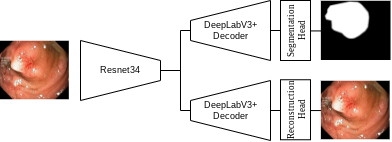
\includegraphics[width=\linewidth]{illustrations/InductiveNet.png}
    \caption{Dual Decoder DeepLabV3}
    \label{fig:dddeeplabv3}
\end{figure}

As will be discussed in Chapter \ref{experiments}, this model also has the advantage of being easily compared to the standard DeepLabV3+; the part of the dual-decoder network responsible for segmentation is after all functionally identical to the single-decoder network.  This facilitates better analysis of the impact of the additional decoder, as the performance of the respective models can be compared directly. 



\section{Consistency as a Surrogate for Generalization}
As discussed in Chapter \ref{background}, distinguishing between generalizable and non-generalizable predictors is not feasible when evaluating only in iid-settings. This is because there is no way of knowing whether the learned features are causally related to the problem, or if they are simply predictive due to some other correlation that is strong in the training domain, but that in practical settings would not have any merit. A \gls{ood}-suitable evaluation procedure therefore requires some way of determining whether the predictor is leveraging non-causal or causal features. Determining what features are causal is, however, an intractable problem. The patterns that neural networks learn are often difficult to identify, and even more difficult to understand intuitively. Moreover, even if these patterns could somehow be understood, it would nonetheless not be possible to determine the causality of the learned features. 

Though establishing what is causal is difficult or even impossible, establishing what \textit{isn't} causal is not all that complicated. To give a concrete example, consider once again the problem of classifying images of cows and camels. Associating the cow class with grass and the camel class with sand is obviously non-causal, since this pattern would not hold if the model for instance is asked to detect cows on Mars or camels on the Moon. To mitigate this, ones first instinct may be to simply collect data of these cows and camels in a wide assortment of differing backgrounds, but such careful curation of datasets is not typically feasible. To give a more concrete example, it is not feasible to collect polyp-segmentation data that is fully representative of all the differing demographics, imaging equipment, operator faults, and so on that one may expect in deployment. There is simply too much variation to be fully accounted for. Instead, one has to be creative with how one uses what data is actually available, and try to squeeze as much utility as possible from it.

Once again going back to the cows and camels example, one may for instance generate multiple instances of the same cow but with varied backgrounds, and in some manner force the model to learn features that are invariant to the backgrounds. This, of course, applies to more than just modifying backgrounds: the more of these non-causal changes to the input data-  from this point on referred to as perturbations - are accounted for and modeled, the more spurious correlations are excluded from the search, and the more likely the model is to learn the patterns that are actually causal. After all, a pattern can for all intents and purposes be considered causal when it holds when subjected to all possible perturbations the model could be exposed to in deployment. 

Though rewarding causal behaviour is intractable, punishing non-causal behaviour is not. All that is required to do so is to be able to apply perturbations that highlight the non-causal reasoning the model employs, quantify the model's sensitivity to these perturbations, then minimize this quantity through optimization. The resulting model will then have learned invariance to whatever causally irrelevant information that the perturbation defines. This property of being invariant to perturbations will be referred to as the consistency of the model. 

Thus, this notion of consistency is in effect a surrogate for generalizability; if a model is consistent to all perturbations, it is invariant to non-causal patterns, and if it is invariant to all non-causal patterns, it necessarily employs causal patterns. Optimizing for consistency can as a result mitigate both shortcut-learning and underspecification, subject only to the span of the space of perturbations and how well inconsistent behaviour can be quantified. For instance, if the perturbations affect the image such that certain shortcuts are broken, these shortcuts are less likely to be learned. A similar argument can be made for underspecification: if multiple predictors are risk equivalent but nevertheless encode conflicting inductive biases, probing the inductive biases learned by the respective predictors through various perturbations can reveal which are generalizable and which are not.

Naturally, this all presupposes that there is some model that can output all possible perturbations one might desire the model to be invariant to. This is of course not the case. As highlighted by the pervasiveness of adversarial attacks and the relative ineffectiveness of adversarial defences, the perturbations that break DNNs are not necesssarily intuitive, and are difficult to analyze in a manner that is conducive to the task of engineering invariances.  

Nevertheless, much stands to be gained if the model learns to be invariant even to a fairly limited space of perturbations. Though generalizability is by no means guaranteed in this case, the odds of learning generalizable features are improved simply because the perturbations limits the types of patterns that a given model can learn. If for instance a white-light endoscopic image is perturbed such that it mimics a narrow-band image, and the model learns to be invariant to this perturbation, predictors that leverage white-light or narrow-band dependent features will no longer be returned from ERM.

This approach, then, requires two components: a perturbation model, and some form of training procedure that imposes invariance to the transformations that the perturbation model employs. 

\subsection{Data Augmentation and Consistency}
    This notion of a perturbation model and modifying the learning objective such that these perturbations are accounted for is not in and of itself a new idea, indeed most deep learning pipeline attempt this implicitly through data augmentation. In this case, the perturbation function is simply randomly applying some set of transformations to the image, and the training procedure is Empirical Risk Minimization. By minimizing the empirical risk subject to a range of augmentation, one might expect that the model will learn features that are optimal across the augmentations being used, and thus endow it with some degree of invariance to these augmentations.
    
    This, however, is not necessarily the case. To illustrate, consider a pipeline intended to segment melanomas. As mentioned in \autoref{gen_failure_med}, the models in such pipelines are often sensitive to skin-tone. Let us assume that the dataset consists primarily of patients with light complexions, and that data augmentation is used in an attempt to combat any bias as a result of this unbalanced dataset. For simplicity, let us assume that the only augmentation used is transforming the image to black-and-white with probability \(p=0.5\). In theory, the empirical risk will be best minimized by learning features that do not consider colour and thus skin-tone at all, and instead simply learn to consider the shapes and sizes of the melanomas. 
    
    This is unlikely for two reasons: first, it presupposes that the model readily learns these generalizable features in favour of the more predictive but spurious features as it is being trained. Second, it assumes that learning to perform well is equally easy on both the augmented and the un-augmented images. If, for instance, the model can quickly achieve high average performance and thus minimize risk by using colour features to achieve excellent performance on the non-augmented images, while exhibiting mediocre performance on the augmented data, it is unlikely that the model will ever exit this extremely broad local minimum in favour of a more shape-biased and generalizable configuration. Moreover, it may be the case that these shape-based features require significantly more parameters in order to model sufficiently and thus that the performance on the augmented data is limited to a much lower upper bound. Thus, risk will be minimized not by learning features invariant to the transform, but by learning features that result in a sufficient equilibrium of performance across the augmented and unaugmented sets. I.e, it will try to learn predictive but brittle features as much as possible to maximize performance on unaugmented data, but under the condition that the performance does not degrade too much on the augmented data This is illustrated in \autoref{fig:melanoma}
    
    \begin{figure}
        \centering
        \includegraphics[width=\linewidth]{example-image-a}
        \caption{Generalization, risk and feature choices}
        \label{fig:melanoma}
    \end{figure}
    
    Thus, a more explicit notion of consistency is required; one that explicitly rewards models that predict equivalently regardless of whether the data is augmented or not, independent of the difficulty of the augmentations, and that weighs the performance on augmented data accordingly. 
    
\subsection{Quantifying Segmentation Consistency}
In the context of segmentation, consistency is the ability of the model to output a reasonably unchanged segmentation when the input data is subjected to some perturbation. One simple approach to express this numerically would simply be to count the number of pixels that do not change in the predictions given some perturbation, and then normalize this with respect to the total number of pixels predicted in both the perturbed and unperturbed images. This, in effect, is equivalent to calculating the \gls{iou} across the perturbed and unperturbed segmentations. However, the ground truth may of course change as a result of the perturbation - if the image is rotated, for example, the segmentation mask should be rotated accordingly. If an image is globally distorted in some way, the segmentation should exhibit the corresponding distortion. This, of course, all needs to be taken into account. This can be achieved by discounting the pixels in the predictions that are expected to change from the overall count. Formally, this metric, referred to as the \glsfirst{sis} can be expressed as follows:

Let \(Y:=\{y,\hat{y}:=f(x)\}\) be the set consisting of the segmentation labels (masks) and predictions for the unperturbed samples, where \(f(\cdot)\) as before denotes the model. Let \(\epsilon(\cdot)\) be some perturbation function - for instance data augmentation. Then, let \(A:=\{a:=\epsilon(y),\hat{a}:=f(\epsilon(x))\}\) be the set consisting of segmentation predictions and masks when the input is subjected to a perturbation. Consistency can then be quantified as:

\begin{equation}
    \mathcal{C}(A,Y) = \frac{\sum\{\{y=1\} \cap \{a=1\} \cap \{\hat{y}=1\} \cap \{\hat{a}=1\} \}}
    {\sum\{\{y=1\} \cup \{a=1\} \cup \{\hat{y}=1\} \cup \{\hat{a}=1\} \}}
\end{equation}

Similarly, \textit{inconsistency} can be expressed using the symmetric difference operator, i.e \(A \ominus B = A \cup B - A \cap B\): 
\begin{equation}\label{sil}
    L_c = \frac{1}{\sum\{y \cup a \cup \hat{y} \cup \hat{a} \}} \sum \{y\ominus\hat{y}\ominus a\ominus\hat{a}\}
\end{equation}

This corresponds to counting the number of pixels that change after the input is subjected to a perturbation - \(\hat{a}\ominus \hat{y}\), but discounting those we expect to change, \(a\ominus y\). 
It should be noted that this metric is minimized not only if the predictions are both correct and consistent with one another, but also if the predictions are both incorrect, so long as whatever change that occurs is consistent with the expected change. This is illustrated in Figure \ref{loss_fn}
\begin{figure}[ht]
    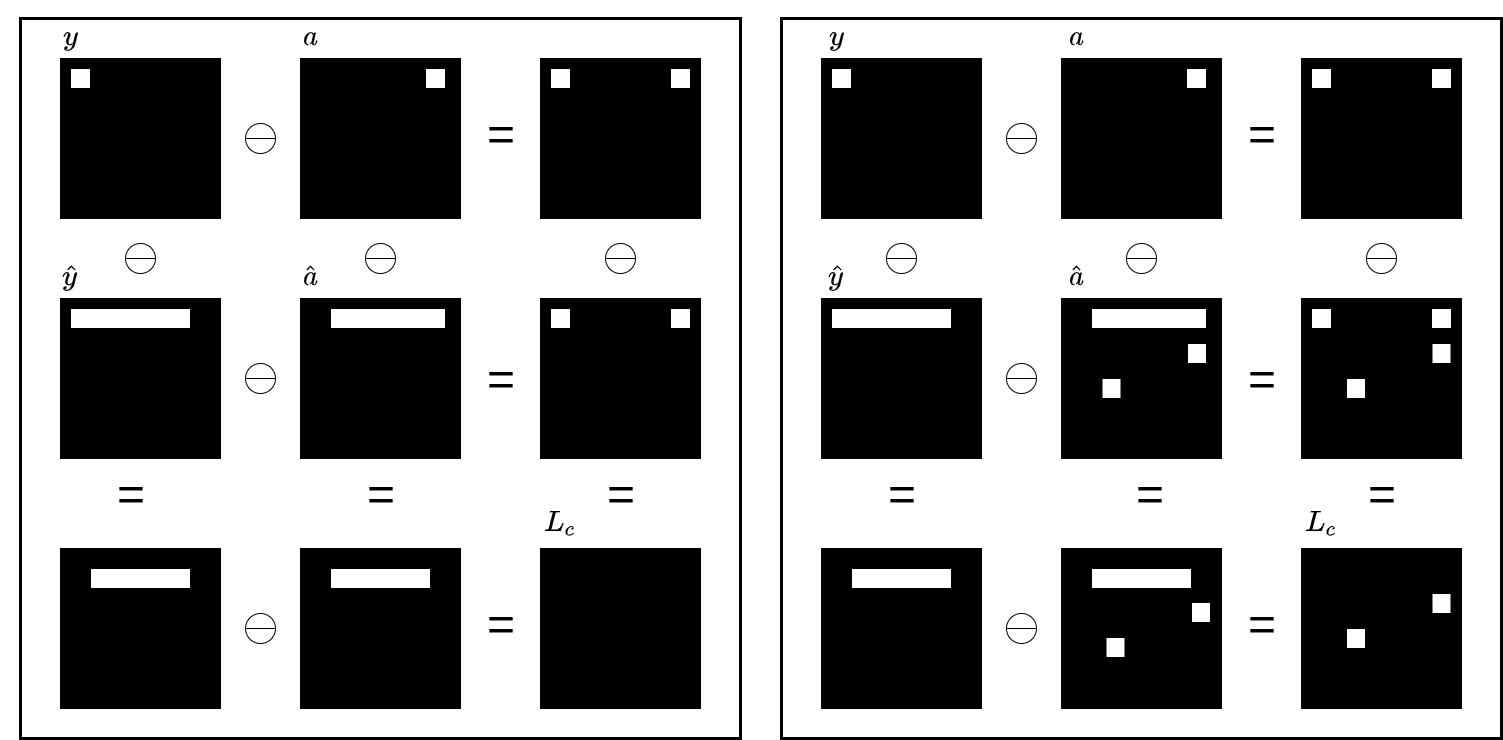
\includegraphics[width=\linewidth]{illustrations/loss_visualisation.drawio.png}
    \caption{Visualisation of \gls{sis} sets, where white is a positive prediction. Note that \gls{sis} is zero regardless of prediction correctness so long as it changes in the expected manner. Note also that the symmetric difference operators are associative. Left shows an instance of consistent and partially incorrect predictions, and right shows an instance of inconsistent and partially correct predictions}
    \label{loss_fn}
\end{figure}  
    
Moreover, note that this metric does not presuppose what transformation has occurred. In Figure \ref{loss_fn}, for instance, the change induced by the perturbation may correspond to simply moving the polyp in the image (and replacing the empty space with a believable background), or it may correspond to a rotation by 90 degrees. How this should be analyzed with respect to consistency is up to interpretation - one can argue that a rotation should rotate the incorrect predictions as well, or one can argue that it should only rotate the correct component of the prediction. For simplicity, \gls{sis} is based on the latter interpretation. This will be discussed in further detail in \autoref{conclusion}

\subsection{Smooth extension and Inconsistency Loss}
Inconsistency as expressed in \autoref{sil} is not differentiable, and thus it cannot in its current state be used as a part of a loss function. This, naturally, limits the utility of the idea somewhat. As such, a smooth extension of this metric in needed. This can be achieved in much the same way as how the Jaccard loss can be derived from the Jaccard index - i.e by using differentiable versions of the set functions. 

I.e, we can extend the definition of the symmetric difference to \(\Theta(A,B) = A(1-B) + B(1-A)\). This, naturally, is equivalent to the standard symmetric difference if the values of A and B are binary. Similarly, the union operator can be extended as \( \bigcup(A,B) = A+B-AB\). Like its binary equivalents, these operators maintain their associative and commutative properties. Consequently, one can optimize for consistency by replacing the operators in \ref{sis} with these functions, which in turn can be used as a loss function:

\begin{equation}
    L_c(y, \hat{y},  a, \hat{a}) = \sum \frac{\Theta(y, \hat{y},  a, \hat{a})}{\bigcup(y, \hat{y},  a, \hat{a})}
\end{equation}

This loss function will from this point be referred to as \glsfirst{sis}. 

\subsection{Mathematical relationship with Data Augmentation}
To prove that training with \gls{sis} indeed is different from simply using data augmentation, one can compare their effects on the gradients. If the gradients are not equal up to scale, training the models will result in exploring different parts of the search-landscape, irrespective of any amount of tuning of learning rates or any of the other hyperparameters governing the optimization process. 

As \gls{sil} is based on the Jaccard index, it will be compared to a pipeline that uses the Jaccard loss. Moreover, since data augmentation is a stochastic process - in other words, the augmentations applied according to some probability \(p\), the gradients can only be analyzed sufficiently by considering the expected loss. 
\begin{align*}
    \mathcal{L} &= \mathbb{E}_p[\mathcal{J}(Z)]; Z \in_{R \thicksim p} \{ \{y, \hat{y}\},\{a, \hat{a}\}\\
    &= p\mathcal{J}(a, \hat{a})+ (1-p)\mathcal{J}(a, \hat{a})
\end{align*}
Thus, the expected gradient is simply:
\begin{equation}
    \nabla \mathcal{L} = p \nabla \mathcal{J}(a, \hat{a})+ (1-p)\nabla \mathcal{J}(a, \hat{a})
\end{equation}
In the case of \gls{sis}:
\begin{align*}
    \mathcal{L} = \sum \frac{\Theta(y, \hat{y},  a, \hat{a})}{\bigcup(y, \hat{y},  a, \hat{a})}
    &=
\end{align*}

\section{Implementing SIS}
So far, it has been assumed that a perturbation model has been given beforehand. This is of course not the case, and naturally any such model needs to be designed with respect to the domain in question. Rotational invariance makes sense for endoscopic images, for instance, but not for classification of hand-written numbers. Thus, in order to engineer such a model, it is first necessary to establish what invariances are desired for the given task. In the case of polyp-segmentation, it is clear that it is necessary to account for variability in for instance lighting, image-resolution, polyp-size, polyp-shape, polyp-location, camera-quality, color-shifts, blurs, optical distortions, and affine transformations. Thus, a model is required that can (more or less) parametrize this variability. Broadly speaking, these transformations can be categorized as follows:
\begin{itemize}
    \item Pixel-wise variability, which affect only the image, i.e color-shifts, brightness shifts, contrast-shifts,  blurs etc. Practically, this corresponds to changes in lighting conditions, camera motion, dye applications, etc.
    \item Geometric variability, which affect both the image and the segmentation mask by some parametrizable quantity, i.e affine transforms and distortions. Practically, this corresponds to endoscope orientation, optical distortion in the camera, zooming, etc. 
    \item Manifold variability, which affects both the image and the segmentation mask depending on a learned model of the distribution. Practically, this corresponds to the size, shape and location of the polyps
\end{itemize}
Pixel-wise variability and geometric variability can be modelled fairly trivially through the use of the same transformations typically used in conventional data-augmentation. Manifold-variability, however, is somewhat more difficult, and requires a functional representation of the distribution. \cite{modelbased} and \cite{cyclegan} achieve this through cross-dataset style-transfer, but this of course necessitates multiple datasets. Given only one dataset, a different method must be used. For a classification task, this could for instance be DeepAugment~\cite{deepaugment} or a similar technique. DeepAugment, however, cannot account for the changes in the segmentation mask that should be induced by the augmentations it generates. Consequently, some other generative model wherein the changes in the segmentation mask can be accounted for is required. To this end, a \gls{gan}-inpainter can be used. 

\subsection{GAN-based Polyp Inpainting}
As mentioned in Chapter \ref{background}, the use of GANs and other distributional modelling in the context of generalization is typically restricted to image-to-image translation, and typically involves transforming an image drawn from one distribution such that it is iid with a second distribution. This, though interesting and no doubt useful assuming several such datasets are available, has limited practical use. It is not necessarily always the case that there exists multiple datasets depicting identical problems, and merely translating between modalities does not as mentioned earlier in the thesis ensure generalizability.

A better approach is to try to model the training set distribution directly, then perturb the data in accordance with this model. For segmentation problems, this can be achieved through training a model to fill some predefined region with pixels that correspond to whatever segmentation target the model is meant to learn, in this case polyps, then perturb a given sample by for instance increasing the size of the polyps or adding extra polyps.

To this end, a simple GAN-inpainter was trained. The Generator \(G(\cdot)\) and Discriminator \(D(\cdot)\) were both based on DeepLabV3Plus, and trained using the following loss formulation, where \(L_d\) and \(L_g\) corresponds to the discriminator and generator loss respectively, and \(x\) and \(y\) corresponds to masked selections of the input image and discriminator labels. 
\begin{align}
    L_g &= 0.001 BCE(D(x),y=1) + 0.999 L1(G(x), x) \\
    L_d &= \frac{1}{2}\big[ BCE(D(G(x),y=1)+BCE(D(G(x), y=0)) \big]
\end{align}

This inpainter was then trained using the Adam optimizer and a cosine annealing scheduler with warm restarts. The following hyperparameters were used:

\begin{tabularx}{\linewidth}{@{}XX@{}}
    \toprule
     Hyperparameter & Value \\
     \midrule
     batch\_size & 8 \\
     learning rate & 0.0001 \\
     epochs & 3000 \\
     Scheduler \(T_0\) & 100\\
     Scheduler \(T_{mult}\) & 2 \\
     \bottomrule
\end{tabularx}

Though this implementation is by no means state-of-the-art, it should nevertheless be sufficient for the purpose of augmentation, considering the principal differences between generated and real polyp images are finer textural details and colour balancing, which are affected by the other augmentations anyway. Figure \ref{fig:inpaint} shows some examples of inpaint, alongside real examples.

\begin{figure}
    \centering
    \includegraphics{example-image-b} 
    \caption{GAN-inpainter rexamples}
    \label{fig:inpaint}
\end{figure}

\subsection{Geometric and pixel-wise transformations}
The data was augmented using the \textit{albumentations} ~\cite{albumentations} library for python, which defines a large number of transformations for use in deep learning. To establish which of these augmentations are suitable, one first needs to establish which invariances the model(s) in question should exhibit. \autoref{tab:vanilla_aug} below provides descriptions of the invariances required in the model, and the albumentation function that corresponds to the required transform. 
\begin{table}[ht]
    \centering
\begin{tabularx}{\textwidth}{|X|X|}
    \toprule
    \textbf{Invariance} & \textbf{Albumentation Function}\\
    \midrule
    Perspective &Flip() \newline RandomRotate90()\\
    Resolution and Zoom & RandomCrop() \\
    Image quality &GaussNoise() \newline ImageCompression()\\
    Camera models&OpticalDistortion() \\
    Lighting conditions & ColorJitter() \\
    \bottomrule
\end{tabularx}
    \caption{Overview of albumentation augmentations}
    \label{tab:vanilla_aug}
\end{table}


The parameters for the respective functions where selected as follows: one transformation was considered at a time, then the maximal parameter value(s) that still kept the polyp visible to an untrained eye were identified. Albumentation augmentations simply use this maximum to perform augmentation. The probability of augmentation was set to 0.5 for all the augmentations with the exception of image compression, which always occured since this transform was defined by a range as opposed to a maximal value. To enable scheduling of augmentation severity, the maximal value was scaled in accordance with a temperature parameter. In the end, this temperature was kept at the maximum, as this was the most conducive to increasing consistency. See the appendix for details. 

\begin{figure}
    \centering
    \includegraphics{example-image-a}
    \caption{Sample Augmentations}
    \label{fig:my_label}
\end{figure}

It should also be noted that this set of augmentations, even including the inpainter, is of course not complete, in the sense that it accounts for all variability that one might expect in practice. As discussed previously it nevertheless may suffice to model a limited space of these transformations, as it increases the likelihood of learning generalizable features. 


\subsection{Consistency Training}

    Similarly to how one can optimize for the Jaccard Index through the Jaccard Loss, so too can one optimize for consistency by using \gls{sis} as a component of a loss function. EXPAND shown in Figure \ref{fig:consistency_training}
    
    \begin{figure}[ht]
            \centering
            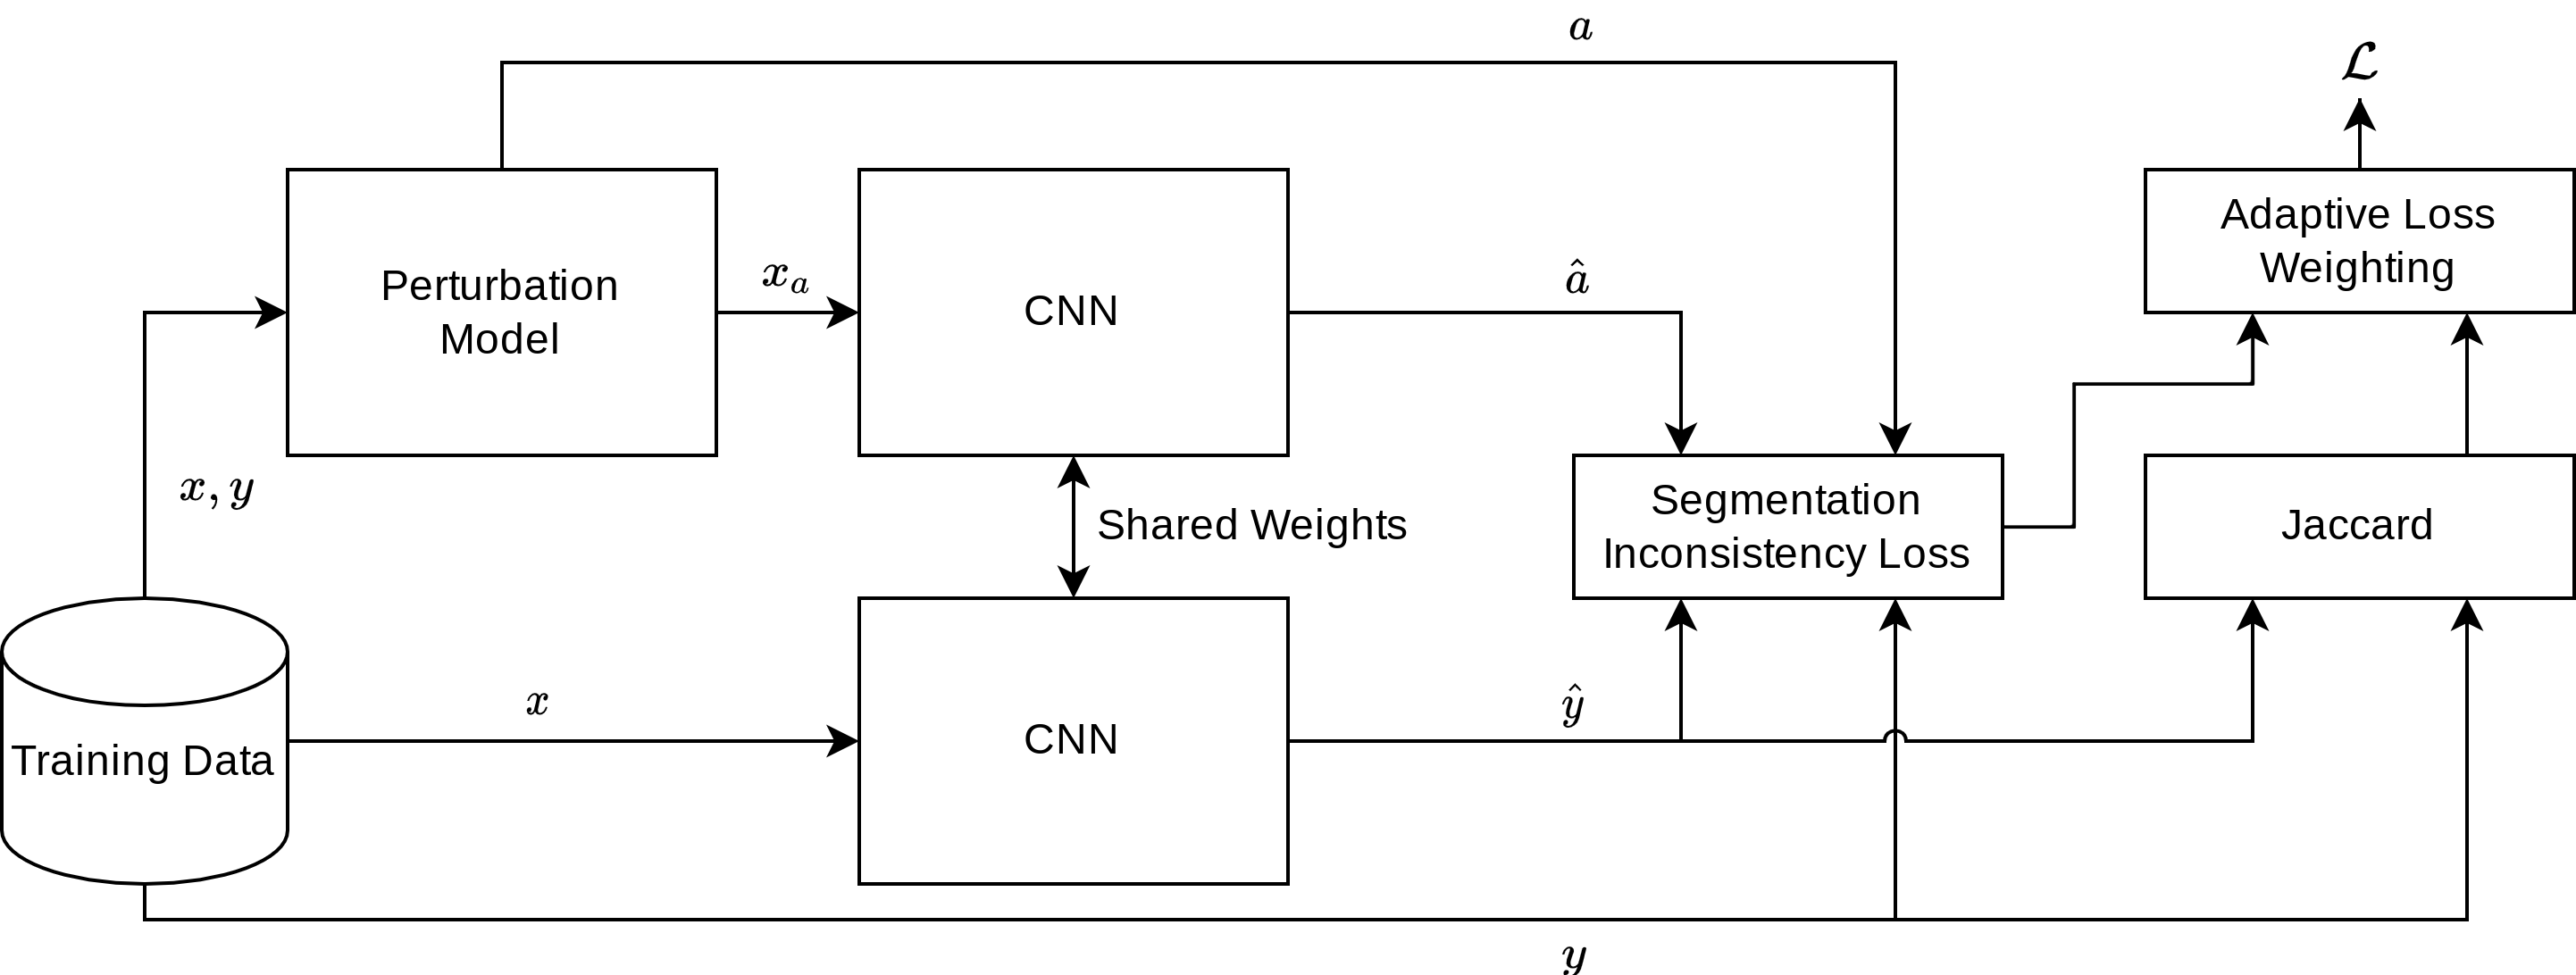
\includegraphics[width=\linewidth]{illustrations/consistency_training.png}
            \caption{Siamese Inconsistency Training}
            \label{fig:consistency_training}
    \end{figure}
    
    Naturally, using \gls{sis} as a loss function on its own is not really useful since it only expresses inconsistency, and is wholly agnostic to whatever object it is trying to segment. Consequently, it has to be combined with a some conventional segmentation loss. A simple way to do this would be to simply add them together and normalize, i.e:
\begin{equation*}
    L(Y, A) = \frac{1}{2} \big[L_{seg}(Y)+L_c(Y,A)\big]
\end{equation*}
Preliminary experiments showed that this, however, exhibited some degree of instability. The model would readily get stuck in local minima where its predictions were indeed consistent, but also consistently predicting artifacts. Examples of this can be found in the appendix. To mitigate this, a better loss function is required. Instead of simply adding the respective losses together, one may weight the individual components adaptively according to the segmentation performance. This way, the model will learn to predict generally correct segmentations early in the training, then start weighing consistency and as a result generalization more and more as the model sees improvements to its segmentation performance:
    \begin{equation}
        L = (1-IoU)\times L_{seg} + IoU \times L_c
    \end{equation}
        If the Jaccard Index (IoU) is used, this is also equivalent to:
    \begin{equation}
        L = {L_{jac}}^2 + (1-L_{jac})L_c
    \end{equation}
Using this formulation, the model will start off trying to learn features that contribute to generally improved segmentation performance, then as segmentation performance improves start principally focusing on learning consistent features. Moreover, if the model starts veering into areas in the loss-landscape that constitute poor segmentation performance, it will self-correct by weighing the segmentation loss more. 

\section{Bayesian Marginalization via Ensembles}

\section{Summary}